\documentclass[10pt]{article}
\usepackage[paperwidth=11in,paperheight=8.5in,margin=.4in,footskip=16pt]{geometry}
\usepackage[T1]{fontenc}\usepackage{lmodern}\usepackage{pgfplots}\usepackage{booktabs}
\pgfplotsset{compat=1.18}\definecolor{navy}{RGB}{25,69,102}
\pagestyle{plain}\setlength{\parindent}{0pt}
\begin{document}
\noindent{\Large\bfseries grid / signals-8-offers-8; American; Symmetric risk aversion (alpha=2); cost multiplier 1}\par\smallskip
{\footnotesize Case: \texttt{grid\_\_signals-8-offers-8\_\_american\_\_ra\_\_cost-1}. Primary profile 1; agreement enabled.}\par\medskip

{\large\bfseries Filing, answering and private exit commitments}\par\smallskip
Filled dots: reached conditional policy. Hollow gray dots: saved off-path policy; the conditional event is undefined.\par
Exit commitments occur privately before the simultaneous agreement decisions.\par\medskip
\begin{tabular}{@{}cc@{}}
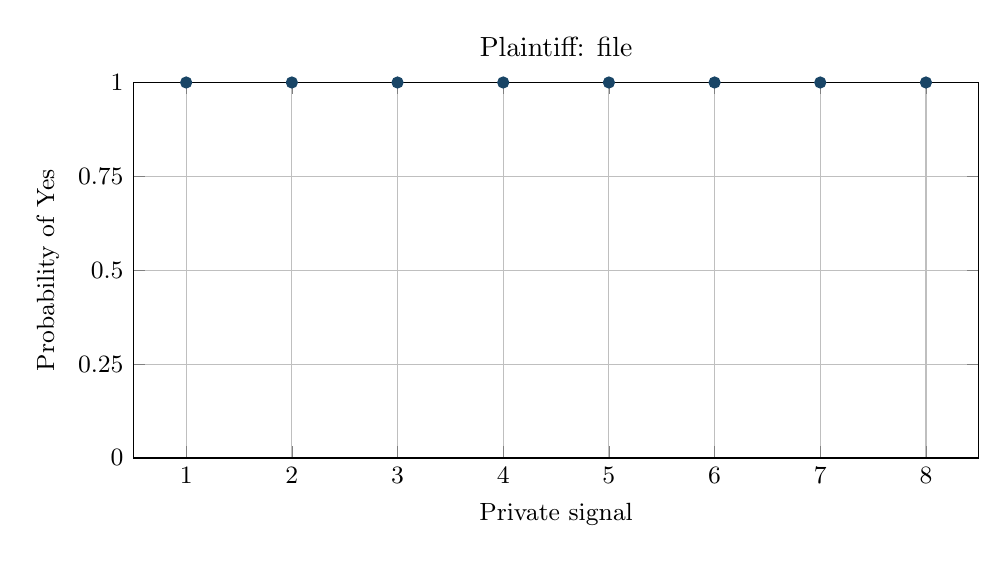
\begin{tikzpicture}\begin{axis}[width=4.85in,height=2.5in,title={Plaintiff: file},xmin=.5,xmax=8.5,ymin=0,ymax=1,xtick={1,...,8},ytick={0,.25,.5,.75,1},xlabel={Private signal},ylabel={Probability of Yes},grid=major,tick label style={font=\small},label style={font=\small},title style={font=\normalsize},clip=false]
\addplot[only marks,mark=*,mark size=2pt,color=navy] coordinates {(1,1) (2,1) (3,1) (4,1) (5,1) (6,1) (7,1) (8,1)};
\addplot[only marks,mark=o,mark size=2.4pt,color=gray] coordinates {};
\end{axis}\end{tikzpicture}&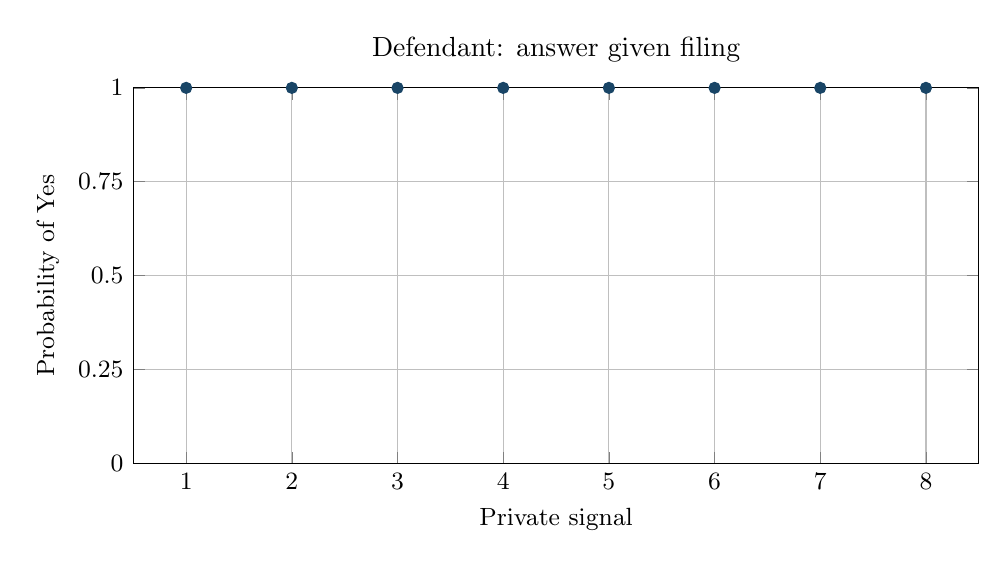
\begin{tikzpicture}\begin{axis}[width=4.85in,height=2.5in,title={Defendant: answer given filing},xmin=.5,xmax=8.5,ymin=0,ymax=1,xtick={1,...,8},ytick={0,.25,.5,.75,1},xlabel={Private signal},ylabel={Probability of Yes},grid=major,tick label style={font=\small},label style={font=\small},title style={font=\normalsize},clip=false]
\addplot[only marks,mark=*,mark size=2pt,color=navy] coordinates {(1,1) (2,1) (3,1) (4,1) (5,1) (6,1) (7,1) (8,1)};
\addplot[only marks,mark=o,mark size=2.4pt,color=gray] coordinates {};
\end{axis}\end{tikzpicture}\\
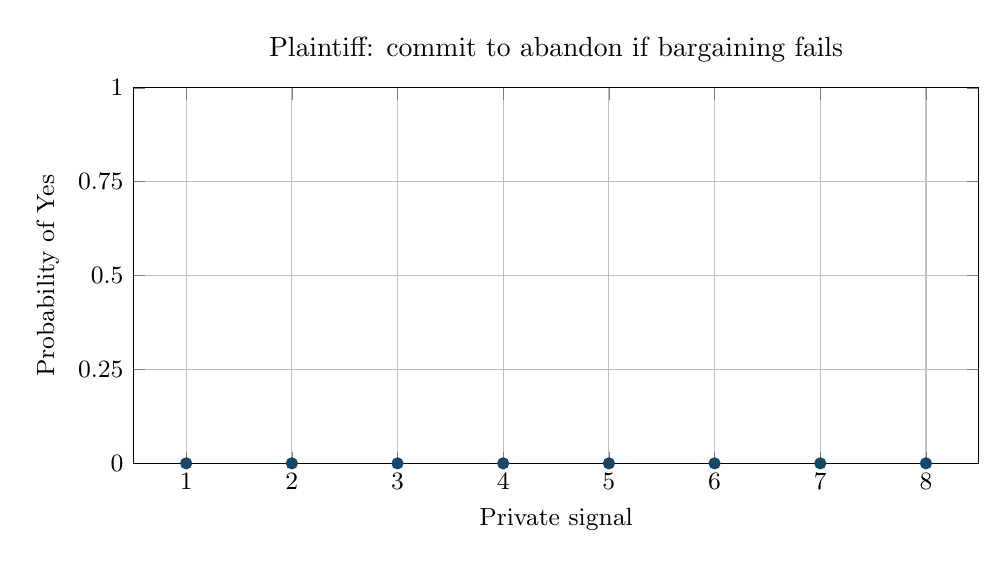
\begin{tikzpicture}\begin{axis}[width=4.85in,height=2.5in,title={Plaintiff: commit to abandon if bargaining fails},xmin=.5,xmax=8.5,ymin=0,ymax=1,xtick={1,...,8},ytick={0,.25,.5,.75,1},xlabel={Private signal},ylabel={Probability of Yes},grid=major,tick label style={font=\small},label style={font=\small},title style={font=\normalsize},clip=false]
\addplot[only marks,mark=*,mark size=2pt,color=navy] coordinates {(1,0) (2,0) (3,0) (4,0) (5,0) (6,0) (7,0) (8,0)};
\addplot[only marks,mark=o,mark size=2.4pt,color=gray] coordinates {};
\end{axis}\end{tikzpicture}&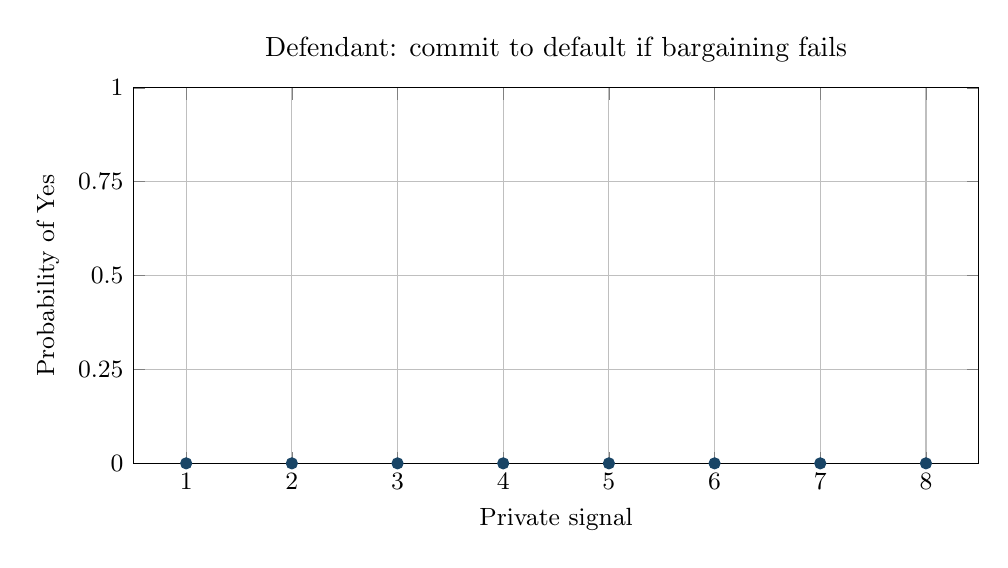
\begin{tikzpicture}\begin{axis}[width=4.85in,height=2.5in,title={Defendant: commit to default if bargaining fails},xmin=.5,xmax=8.5,ymin=0,ymax=1,xtick={1,...,8},ytick={0,.25,.5,.75,1},xlabel={Private signal},ylabel={Probability of Yes},grid=major,tick label style={font=\small},label style={font=\small},title style={font=\normalsize},clip=false]
\addplot[only marks,mark=*,mark size=2pt,color=navy] coordinates {(1,0) (2,0) (3,0) (4,0) (5,0) (6,0) (7,0) (8,0)};
\addplot[only marks,mark=o,mark size=2.4pt,color=gray] coordinates {};
\end{axis}\end{tikzpicture}
\end{tabular}\par\smallskip
{\small Filing: 1; joint filing/answering: 1; answering given filing: 1.}

\newpage
\noindent{\Large\bfseries grid / signals-8-offers-8; American; Symmetric risk aversion (alpha=2); cost multiplier 1}\par\smallskip
{\footnotesize Case: \texttt{grid\_\_signals-8-offers-8\_\_american\_\_ra\_\_cost-1}. Primary profile 1; agreement enabled.}\par\medskip

{\large\bfseries Agreement conditional on private signal and own exit commitment}\par\smallskip
Both parties choose without observing the other party\textquotesingle s agreement choice or private exit commitment.\par
Offers occur only if both agree. Refusal activates the original commitment-dependent outcomes.\par\medskip
\begin{tabular}{@{}cc@{}}
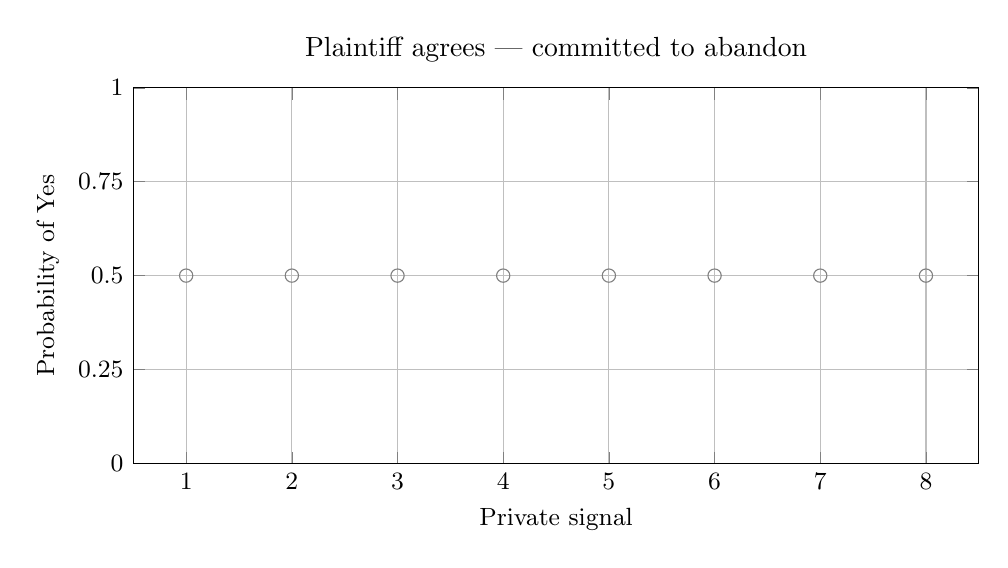
\begin{tikzpicture}\begin{axis}[width=4.85in,height=2.5in,title={Plaintiff agrees | committed to abandon},xmin=.5,xmax=8.5,ymin=0,ymax=1,xtick={1,...,8},ytick={0,.25,.5,.75,1},xlabel={Private signal},ylabel={Probability of Yes},grid=major,tick label style={font=\small},label style={font=\small},title style={font=\normalsize},clip=false]
\addplot[only marks,mark=*,mark size=2pt,color=navy] coordinates {};
\addplot[only marks,mark=o,mark size=2.4pt,color=gray] coordinates {(1,0.5) (2,0.5) (3,0.5) (4,0.5) (5,0.5) (6,0.5) (7,0.5) (8,0.5)};
\end{axis}\end{tikzpicture}&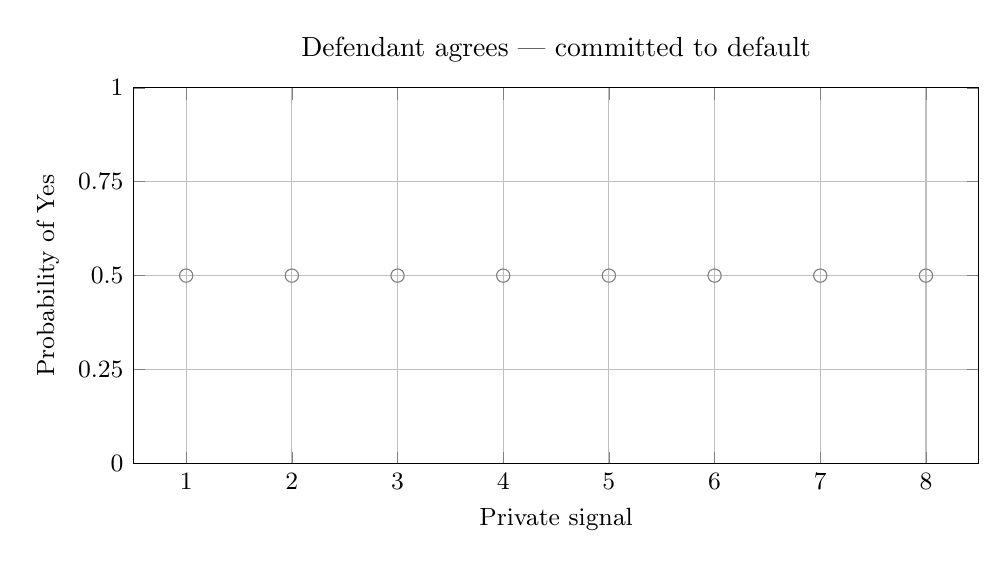
\begin{tikzpicture}\begin{axis}[width=4.85in,height=2.5in,title={Defendant agrees | committed to default},xmin=.5,xmax=8.5,ymin=0,ymax=1,xtick={1,...,8},ytick={0,.25,.5,.75,1},xlabel={Private signal},ylabel={Probability of Yes},grid=major,tick label style={font=\small},label style={font=\small},title style={font=\normalsize},clip=false]
\addplot[only marks,mark=*,mark size=2pt,color=navy] coordinates {};
\addplot[only marks,mark=o,mark size=2.4pt,color=gray] coordinates {(1,0.5) (2,0.5) (3,0.5) (4,0.5) (5,0.5) (6,0.5) (7,0.5) (8,0.5)};
\end{axis}\end{tikzpicture}\\
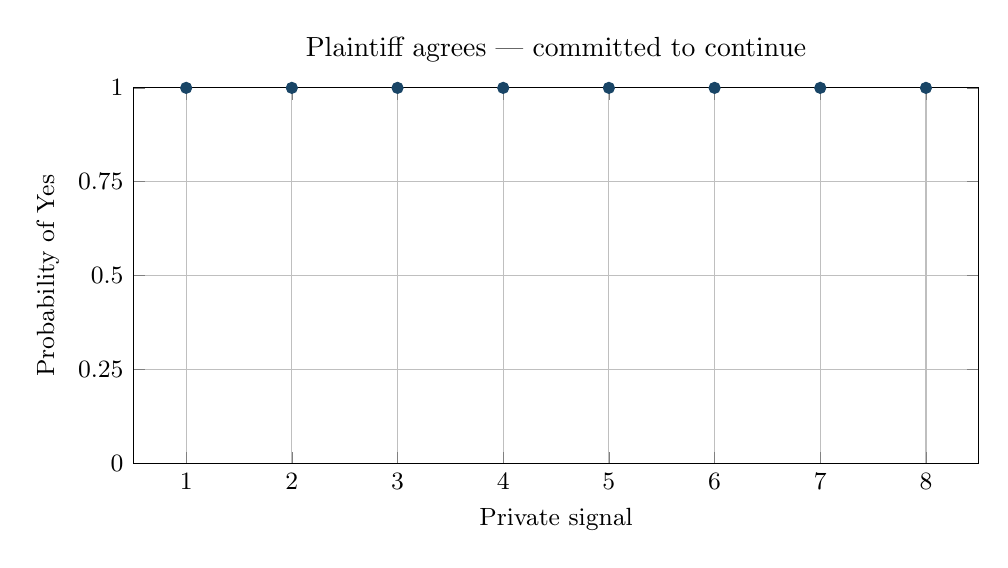
\begin{tikzpicture}\begin{axis}[width=4.85in,height=2.5in,title={Plaintiff agrees | committed to continue},xmin=.5,xmax=8.5,ymin=0,ymax=1,xtick={1,...,8},ytick={0,.25,.5,.75,1},xlabel={Private signal},ylabel={Probability of Yes},grid=major,tick label style={font=\small},label style={font=\small},title style={font=\normalsize},clip=false]
\addplot[only marks,mark=*,mark size=2pt,color=navy] coordinates {(1,1) (2,1) (3,1) (4,1) (5,1) (6,1) (7,1) (8,1)};
\addplot[only marks,mark=o,mark size=2.4pt,color=gray] coordinates {};
\end{axis}\end{tikzpicture}&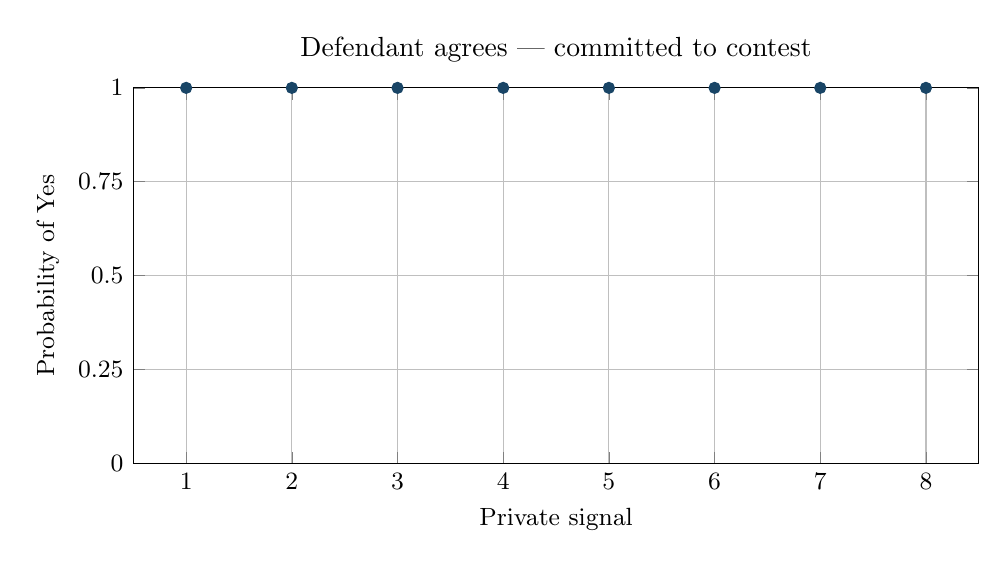
\begin{tikzpicture}\begin{axis}[width=4.85in,height=2.5in,title={Defendant agrees | committed to contest},xmin=.5,xmax=8.5,ymin=0,ymax=1,xtick={1,...,8},ytick={0,.25,.5,.75,1},xlabel={Private signal},ylabel={Probability of Yes},grid=major,tick label style={font=\small},label style={font=\small},title style={font=\normalsize},clip=false]
\addplot[only marks,mark=*,mark size=2pt,color=navy] coordinates {(1,1) (2,1) (3,1) (4,1) (5,1) (6,1) (7,1) (8,1)};
\addplot[only marks,mark=o,mark size=2.4pt,color=gray] coordinates {};
\end{axis}\end{tikzpicture}
\end{tabular}\par\smallskip
{\small Joint agreement-stage reach: 1. Conditional joint outcomes: both agree 1; only P declines 0; only D declines 0; both decline 0. These use the full joint signal/history distribution. Hollow dots retain saved off-path policies.}
\newpage
\noindent{\Large\bfseries grid / signals-8-offers-8; American; Symmetric risk aversion (alpha=2); cost multiplier 1}\par\smallskip
{\footnotesize Case: \texttt{grid\_\_signals-8-offers-8\_\_american\_\_ra\_\_cost-1}. Primary profile 1; agreement enabled.}\par\medskip

{\large\bfseries Complete mixed offer distributions}\par\smallskip
Rows show the saved policy at each private signal and own commitment, after both parties agree to bargain.\par
An asterisk marks an unreachable information set: its saved completion is shown, but no reached conditional distribution exists.\par\medskip
\begin{tabular}{@{}cc@{}}
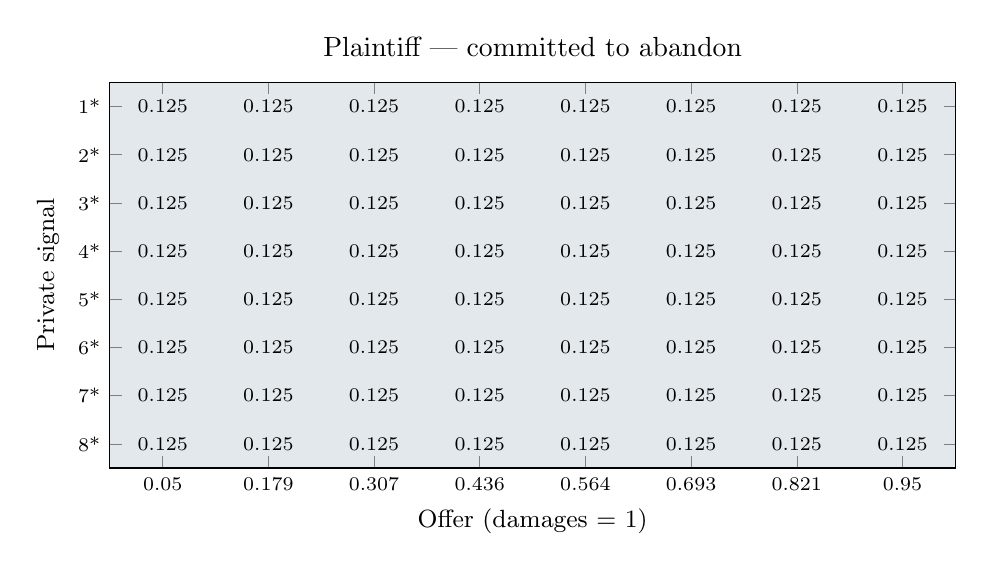
\begin{tikzpicture}\begin{axis}[
width=4.85in,height=2.55in,title={Plaintiff | committed to abandon},
xmin=.5,xmax=8.5,ymin=.5,ymax=8.5,y dir=reverse,
xtick={1,...,8},xticklabels={0.05,0.179,0.307,0.436,0.564,0.693,0.821,0.95},
ytick={1,...,8},yticklabels={1*,2*,3*,4*,5*,6*,7*,8*},
xlabel={Offer (damages = 1)},ylabel={Private signal},
tick label style={font=\scriptsize},label style={font=\small},title style={font=\normalsize},
colormap={policy}{color(0cm)=(white);color(1cm)=(navy)},point meta min=0,point meta max=1,
axis on top,clip=false]
\addplot[matrix plot*,mesh/cols=8,point meta=explicit] table[meta=p] {
x y p
1 1 0.125
2 1 0.125
3 1 0.125
4 1 0.125
5 1 0.125
6 1 0.125
7 1 0.125
8 1 0.125
1 2 0.125
2 2 0.125
3 2 0.125
4 2 0.125
5 2 0.125
6 2 0.125
7 2 0.125
8 2 0.125
1 3 0.125
2 3 0.125
3 3 0.125
4 3 0.125
5 3 0.125
6 3 0.125
7 3 0.125
8 3 0.125
1 4 0.125
2 4 0.125
3 4 0.125
4 4 0.125
5 4 0.125
6 4 0.125
7 4 0.125
8 4 0.125
1 5 0.125
2 5 0.125
3 5 0.125
4 5 0.125
5 5 0.125
6 5 0.125
7 5 0.125
8 5 0.125
1 6 0.125
2 6 0.125
3 6 0.125
4 6 0.125
5 6 0.125
6 6 0.125
7 6 0.125
8 6 0.125
1 7 0.125
2 7 0.125
3 7 0.125
4 7 0.125
5 7 0.125
6 7 0.125
7 7 0.125
8 7 0.125
1 8 0.125
2 8 0.125
3 8 0.125
4 8 0.125
5 8 0.125
6 8 0.125
7 8 0.125
8 8 0.125
};
\node[font=\scriptsize,text=black] at (axis cs:1,1) {0.125};
\node[font=\scriptsize,text=black] at (axis cs:2,1) {0.125};
\node[font=\scriptsize,text=black] at (axis cs:3,1) {0.125};
\node[font=\scriptsize,text=black] at (axis cs:4,1) {0.125};
\node[font=\scriptsize,text=black] at (axis cs:5,1) {0.125};
\node[font=\scriptsize,text=black] at (axis cs:6,1) {0.125};
\node[font=\scriptsize,text=black] at (axis cs:7,1) {0.125};
\node[font=\scriptsize,text=black] at (axis cs:8,1) {0.125};
\node[font=\scriptsize,text=black] at (axis cs:1,2) {0.125};
\node[font=\scriptsize,text=black] at (axis cs:2,2) {0.125};
\node[font=\scriptsize,text=black] at (axis cs:3,2) {0.125};
\node[font=\scriptsize,text=black] at (axis cs:4,2) {0.125};
\node[font=\scriptsize,text=black] at (axis cs:5,2) {0.125};
\node[font=\scriptsize,text=black] at (axis cs:6,2) {0.125};
\node[font=\scriptsize,text=black] at (axis cs:7,2) {0.125};
\node[font=\scriptsize,text=black] at (axis cs:8,2) {0.125};
\node[font=\scriptsize,text=black] at (axis cs:1,3) {0.125};
\node[font=\scriptsize,text=black] at (axis cs:2,3) {0.125};
\node[font=\scriptsize,text=black] at (axis cs:3,3) {0.125};
\node[font=\scriptsize,text=black] at (axis cs:4,3) {0.125};
\node[font=\scriptsize,text=black] at (axis cs:5,3) {0.125};
\node[font=\scriptsize,text=black] at (axis cs:6,3) {0.125};
\node[font=\scriptsize,text=black] at (axis cs:7,3) {0.125};
\node[font=\scriptsize,text=black] at (axis cs:8,3) {0.125};
\node[font=\scriptsize,text=black] at (axis cs:1,4) {0.125};
\node[font=\scriptsize,text=black] at (axis cs:2,4) {0.125};
\node[font=\scriptsize,text=black] at (axis cs:3,4) {0.125};
\node[font=\scriptsize,text=black] at (axis cs:4,4) {0.125};
\node[font=\scriptsize,text=black] at (axis cs:5,4) {0.125};
\node[font=\scriptsize,text=black] at (axis cs:6,4) {0.125};
\node[font=\scriptsize,text=black] at (axis cs:7,4) {0.125};
\node[font=\scriptsize,text=black] at (axis cs:8,4) {0.125};
\node[font=\scriptsize,text=black] at (axis cs:1,5) {0.125};
\node[font=\scriptsize,text=black] at (axis cs:2,5) {0.125};
\node[font=\scriptsize,text=black] at (axis cs:3,5) {0.125};
\node[font=\scriptsize,text=black] at (axis cs:4,5) {0.125};
\node[font=\scriptsize,text=black] at (axis cs:5,5) {0.125};
\node[font=\scriptsize,text=black] at (axis cs:6,5) {0.125};
\node[font=\scriptsize,text=black] at (axis cs:7,5) {0.125};
\node[font=\scriptsize,text=black] at (axis cs:8,5) {0.125};
\node[font=\scriptsize,text=black] at (axis cs:1,6) {0.125};
\node[font=\scriptsize,text=black] at (axis cs:2,6) {0.125};
\node[font=\scriptsize,text=black] at (axis cs:3,6) {0.125};
\node[font=\scriptsize,text=black] at (axis cs:4,6) {0.125};
\node[font=\scriptsize,text=black] at (axis cs:5,6) {0.125};
\node[font=\scriptsize,text=black] at (axis cs:6,6) {0.125};
\node[font=\scriptsize,text=black] at (axis cs:7,6) {0.125};
\node[font=\scriptsize,text=black] at (axis cs:8,6) {0.125};
\node[font=\scriptsize,text=black] at (axis cs:1,7) {0.125};
\node[font=\scriptsize,text=black] at (axis cs:2,7) {0.125};
\node[font=\scriptsize,text=black] at (axis cs:3,7) {0.125};
\node[font=\scriptsize,text=black] at (axis cs:4,7) {0.125};
\node[font=\scriptsize,text=black] at (axis cs:5,7) {0.125};
\node[font=\scriptsize,text=black] at (axis cs:6,7) {0.125};
\node[font=\scriptsize,text=black] at (axis cs:7,7) {0.125};
\node[font=\scriptsize,text=black] at (axis cs:8,7) {0.125};
\node[font=\scriptsize,text=black] at (axis cs:1,8) {0.125};
\node[font=\scriptsize,text=black] at (axis cs:2,8) {0.125};
\node[font=\scriptsize,text=black] at (axis cs:3,8) {0.125};
\node[font=\scriptsize,text=black] at (axis cs:4,8) {0.125};
\node[font=\scriptsize,text=black] at (axis cs:5,8) {0.125};
\node[font=\scriptsize,text=black] at (axis cs:6,8) {0.125};
\node[font=\scriptsize,text=black] at (axis cs:7,8) {0.125};
\node[font=\scriptsize,text=black] at (axis cs:8,8) {0.125};
\end{axis}\end{tikzpicture}&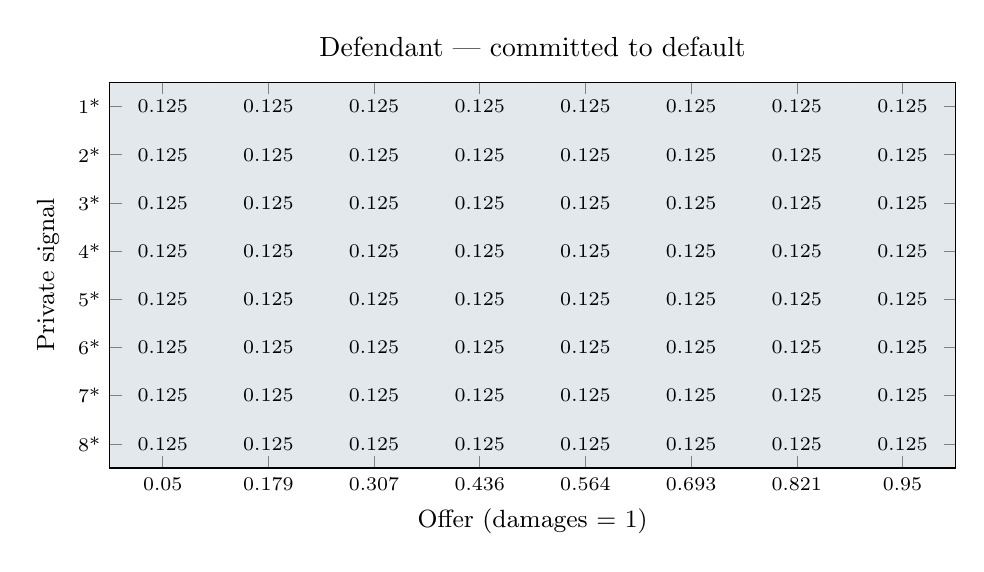
\begin{tikzpicture}\begin{axis}[
width=4.85in,height=2.55in,title={Defendant | committed to default},
xmin=.5,xmax=8.5,ymin=.5,ymax=8.5,y dir=reverse,
xtick={1,...,8},xticklabels={0.05,0.179,0.307,0.436,0.564,0.693,0.821,0.95},
ytick={1,...,8},yticklabels={1*,2*,3*,4*,5*,6*,7*,8*},
xlabel={Offer (damages = 1)},ylabel={Private signal},
tick label style={font=\scriptsize},label style={font=\small},title style={font=\normalsize},
colormap={policy}{color(0cm)=(white);color(1cm)=(navy)},point meta min=0,point meta max=1,
axis on top,clip=false]
\addplot[matrix plot*,mesh/cols=8,point meta=explicit] table[meta=p] {
x y p
1 1 0.125
2 1 0.125
3 1 0.125
4 1 0.125
5 1 0.125
6 1 0.125
7 1 0.125
8 1 0.125
1 2 0.125
2 2 0.125
3 2 0.125
4 2 0.125
5 2 0.125
6 2 0.125
7 2 0.125
8 2 0.125
1 3 0.125
2 3 0.125
3 3 0.125
4 3 0.125
5 3 0.125
6 3 0.125
7 3 0.125
8 3 0.125
1 4 0.125
2 4 0.125
3 4 0.125
4 4 0.125
5 4 0.125
6 4 0.125
7 4 0.125
8 4 0.125
1 5 0.125
2 5 0.125
3 5 0.125
4 5 0.125
5 5 0.125
6 5 0.125
7 5 0.125
8 5 0.125
1 6 0.125
2 6 0.125
3 6 0.125
4 6 0.125
5 6 0.125
6 6 0.125
7 6 0.125
8 6 0.125
1 7 0.125
2 7 0.125
3 7 0.125
4 7 0.125
5 7 0.125
6 7 0.125
7 7 0.125
8 7 0.125
1 8 0.125
2 8 0.125
3 8 0.125
4 8 0.125
5 8 0.125
6 8 0.125
7 8 0.125
8 8 0.125
};
\node[font=\scriptsize,text=black] at (axis cs:1,1) {0.125};
\node[font=\scriptsize,text=black] at (axis cs:2,1) {0.125};
\node[font=\scriptsize,text=black] at (axis cs:3,1) {0.125};
\node[font=\scriptsize,text=black] at (axis cs:4,1) {0.125};
\node[font=\scriptsize,text=black] at (axis cs:5,1) {0.125};
\node[font=\scriptsize,text=black] at (axis cs:6,1) {0.125};
\node[font=\scriptsize,text=black] at (axis cs:7,1) {0.125};
\node[font=\scriptsize,text=black] at (axis cs:8,1) {0.125};
\node[font=\scriptsize,text=black] at (axis cs:1,2) {0.125};
\node[font=\scriptsize,text=black] at (axis cs:2,2) {0.125};
\node[font=\scriptsize,text=black] at (axis cs:3,2) {0.125};
\node[font=\scriptsize,text=black] at (axis cs:4,2) {0.125};
\node[font=\scriptsize,text=black] at (axis cs:5,2) {0.125};
\node[font=\scriptsize,text=black] at (axis cs:6,2) {0.125};
\node[font=\scriptsize,text=black] at (axis cs:7,2) {0.125};
\node[font=\scriptsize,text=black] at (axis cs:8,2) {0.125};
\node[font=\scriptsize,text=black] at (axis cs:1,3) {0.125};
\node[font=\scriptsize,text=black] at (axis cs:2,3) {0.125};
\node[font=\scriptsize,text=black] at (axis cs:3,3) {0.125};
\node[font=\scriptsize,text=black] at (axis cs:4,3) {0.125};
\node[font=\scriptsize,text=black] at (axis cs:5,3) {0.125};
\node[font=\scriptsize,text=black] at (axis cs:6,3) {0.125};
\node[font=\scriptsize,text=black] at (axis cs:7,3) {0.125};
\node[font=\scriptsize,text=black] at (axis cs:8,3) {0.125};
\node[font=\scriptsize,text=black] at (axis cs:1,4) {0.125};
\node[font=\scriptsize,text=black] at (axis cs:2,4) {0.125};
\node[font=\scriptsize,text=black] at (axis cs:3,4) {0.125};
\node[font=\scriptsize,text=black] at (axis cs:4,4) {0.125};
\node[font=\scriptsize,text=black] at (axis cs:5,4) {0.125};
\node[font=\scriptsize,text=black] at (axis cs:6,4) {0.125};
\node[font=\scriptsize,text=black] at (axis cs:7,4) {0.125};
\node[font=\scriptsize,text=black] at (axis cs:8,4) {0.125};
\node[font=\scriptsize,text=black] at (axis cs:1,5) {0.125};
\node[font=\scriptsize,text=black] at (axis cs:2,5) {0.125};
\node[font=\scriptsize,text=black] at (axis cs:3,5) {0.125};
\node[font=\scriptsize,text=black] at (axis cs:4,5) {0.125};
\node[font=\scriptsize,text=black] at (axis cs:5,5) {0.125};
\node[font=\scriptsize,text=black] at (axis cs:6,5) {0.125};
\node[font=\scriptsize,text=black] at (axis cs:7,5) {0.125};
\node[font=\scriptsize,text=black] at (axis cs:8,5) {0.125};
\node[font=\scriptsize,text=black] at (axis cs:1,6) {0.125};
\node[font=\scriptsize,text=black] at (axis cs:2,6) {0.125};
\node[font=\scriptsize,text=black] at (axis cs:3,6) {0.125};
\node[font=\scriptsize,text=black] at (axis cs:4,6) {0.125};
\node[font=\scriptsize,text=black] at (axis cs:5,6) {0.125};
\node[font=\scriptsize,text=black] at (axis cs:6,6) {0.125};
\node[font=\scriptsize,text=black] at (axis cs:7,6) {0.125};
\node[font=\scriptsize,text=black] at (axis cs:8,6) {0.125};
\node[font=\scriptsize,text=black] at (axis cs:1,7) {0.125};
\node[font=\scriptsize,text=black] at (axis cs:2,7) {0.125};
\node[font=\scriptsize,text=black] at (axis cs:3,7) {0.125};
\node[font=\scriptsize,text=black] at (axis cs:4,7) {0.125};
\node[font=\scriptsize,text=black] at (axis cs:5,7) {0.125};
\node[font=\scriptsize,text=black] at (axis cs:6,7) {0.125};
\node[font=\scriptsize,text=black] at (axis cs:7,7) {0.125};
\node[font=\scriptsize,text=black] at (axis cs:8,7) {0.125};
\node[font=\scriptsize,text=black] at (axis cs:1,8) {0.125};
\node[font=\scriptsize,text=black] at (axis cs:2,8) {0.125};
\node[font=\scriptsize,text=black] at (axis cs:3,8) {0.125};
\node[font=\scriptsize,text=black] at (axis cs:4,8) {0.125};
\node[font=\scriptsize,text=black] at (axis cs:5,8) {0.125};
\node[font=\scriptsize,text=black] at (axis cs:6,8) {0.125};
\node[font=\scriptsize,text=black] at (axis cs:7,8) {0.125};
\node[font=\scriptsize,text=black] at (axis cs:8,8) {0.125};
\end{axis}\end{tikzpicture}\\
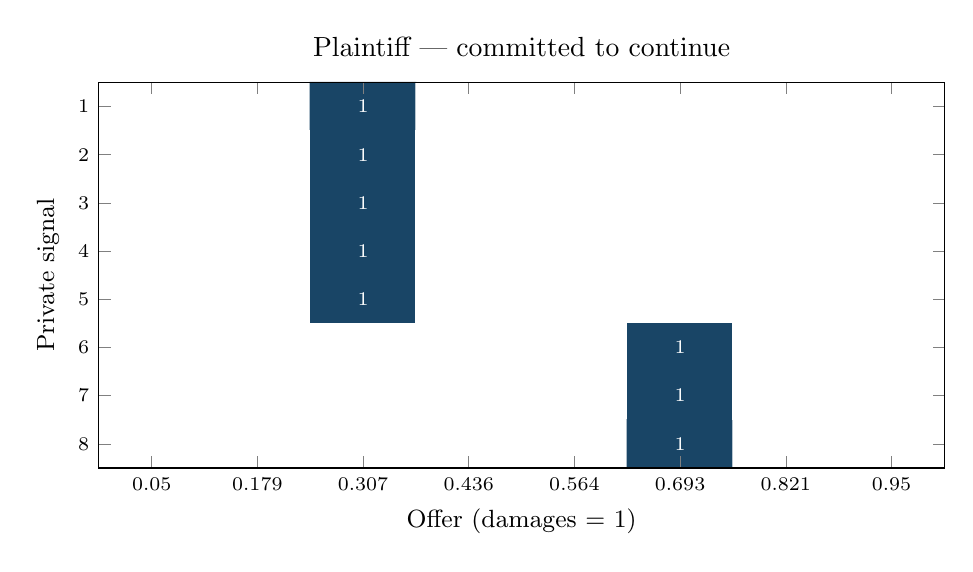
\begin{tikzpicture}\begin{axis}[
width=4.85in,height=2.55in,title={Plaintiff | committed to continue},
xmin=.5,xmax=8.5,ymin=.5,ymax=8.5,y dir=reverse,
xtick={1,...,8},xticklabels={0.05,0.179,0.307,0.436,0.564,0.693,0.821,0.95},
ytick={1,...,8},yticklabels={1,2,3,4,5,6,7,8},
xlabel={Offer (damages = 1)},ylabel={Private signal},
tick label style={font=\scriptsize},label style={font=\small},title style={font=\normalsize},
colormap={policy}{color(0cm)=(white);color(1cm)=(navy)},point meta min=0,point meta max=1,
axis on top,clip=false]
\addplot[matrix plot*,mesh/cols=8,point meta=explicit] table[meta=p] {
x y p
1 1 0
2 1 0
3 1 1
4 1 0
5 1 0
6 1 0
7 1 0
8 1 0
1 2 0
2 2 0
3 2 1
4 2 0
5 2 0
6 2 0
7 2 0
8 2 0
1 3 0
2 3 0
3 3 1
4 3 0
5 3 0
6 3 0
7 3 0
8 3 0
1 4 0
2 4 0
3 4 1
4 4 0
5 4 0
6 4 0
7 4 0
8 4 0
1 5 0
2 5 0
3 5 1
4 5 0
5 5 0
6 5 0
7 5 0
8 5 0
1 6 0
2 6 0
3 6 0
4 6 0
5 6 0
6 6 1
7 6 0
8 6 0
1 7 0
2 7 0
3 7 0
4 7 0
5 7 0
6 7 1
7 7 0
8 7 0
1 8 0
2 8 0
3 8 0
4 8 0
5 8 0
6 8 1
7 8 0
8 8 0
};
\node[font=\scriptsize,text=white] at (axis cs:3,1) {1};
\node[font=\scriptsize,text=white] at (axis cs:3,2) {1};
\node[font=\scriptsize,text=white] at (axis cs:3,3) {1};
\node[font=\scriptsize,text=white] at (axis cs:3,4) {1};
\node[font=\scriptsize,text=white] at (axis cs:3,5) {1};
\node[font=\scriptsize,text=white] at (axis cs:6,6) {1};
\node[font=\scriptsize,text=white] at (axis cs:6,7) {1};
\node[font=\scriptsize,text=white] at (axis cs:6,8) {1};
\end{axis}\end{tikzpicture}&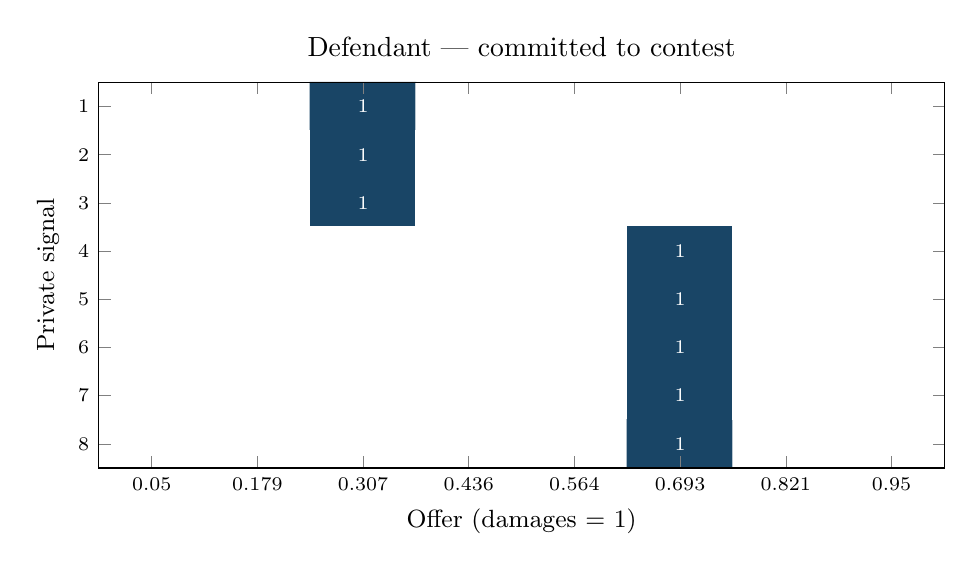
\begin{tikzpicture}\begin{axis}[
width=4.85in,height=2.55in,title={Defendant | committed to contest},
xmin=.5,xmax=8.5,ymin=.5,ymax=8.5,y dir=reverse,
xtick={1,...,8},xticklabels={0.05,0.179,0.307,0.436,0.564,0.693,0.821,0.95},
ytick={1,...,8},yticklabels={1,2,3,4,5,6,7,8},
xlabel={Offer (damages = 1)},ylabel={Private signal},
tick label style={font=\scriptsize},label style={font=\small},title style={font=\normalsize},
colormap={policy}{color(0cm)=(white);color(1cm)=(navy)},point meta min=0,point meta max=1,
axis on top,clip=false]
\addplot[matrix plot*,mesh/cols=8,point meta=explicit] table[meta=p] {
x y p
1 1 0
2 1 0
3 1 1
4 1 0
5 1 0
6 1 0
7 1 0
8 1 0
1 2 0
2 2 0
3 2 1
4 2 0
5 2 0
6 2 0
7 2 0
8 2 0
1 3 0
2 3 0
3 3 1
4 3 0
5 3 0
6 3 0
7 3 0
8 3 0
1 4 0
2 4 0
3 4 0
4 4 0
5 4 0
6 4 1
7 4 0
8 4 0
1 5 0
2 5 0
3 5 0
4 5 0
5 5 0
6 5 1
7 5 0
8 5 0
1 6 0
2 6 0
3 6 0
4 6 0
5 6 0
6 6 1
7 6 0
8 6 0
1 7 0
2 7 0
3 7 0
4 7 0
5 7 0
6 7 1
7 7 0
8 7 0
1 8 0
2 8 0
3 8 0
4 8 0
5 8 0
6 8 1
7 8 0
8 8 0
};
\node[font=\scriptsize,text=white] at (axis cs:3,1) {1};
\node[font=\scriptsize,text=white] at (axis cs:3,2) {1};
\node[font=\scriptsize,text=white] at (axis cs:3,3) {1};
\node[font=\scriptsize,text=white] at (axis cs:6,4) {1};
\node[font=\scriptsize,text=white] at (axis cs:6,5) {1};
\node[font=\scriptsize,text=white] at (axis cs:6,6) {1};
\node[font=\scriptsize,text=white] at (axis cs:6,7) {1};
\node[font=\scriptsize,text=white] at (axis cs:6,8) {1};
\end{axis}\end{tikzpicture}
\end{tabular}\par\smallskip
{\small Color and cell labels show action probabilities (white = 0; darkest blue = 1). Empty cell labels mean exact zero.
Every positive entry is printed, including arbitrarily small probabilities. Full precision is retained in the editable TeX and profile JSON.}
\end{document}